%
% Draft  document skinspace.tex
% Looks at how follicle development may affect expansion of the skin
%
 
\documentclass[titlepage]{article}  % Latex2e
\usepackage{graphicx,lscape,subfigure}
\usepackage{tikz}
\usepackage{bm,longtable}
\usepackage{textcomp}
 

\title{Does follicle development affect the spatial layout of sheep skin?}
\author{Neville Jackson and Jim Watts}
\date{27 Jan 2018} 

 
\begin{document} 


 
\maketitle      
\tableofcontents

$\newcommand{\E}{\mathrm{E}}$
$\newcommand{\Var}{\mathrm{Var}}$
$\newcommand{\Cov}{\mathrm{Cov}}$ 
$\newcommand{\SD}{\mathrm{SD}}$ 

\clearpage
\section{Introduction} 
 An attempt was made , in Jackson and Watts(2017)~\cite{jack:17b} to put forward the hypothesis that wrinkles form in the foetus at the same stage as secondary follicle development so would be likely to affect secondary follicle density or S/P ratio or secondary fibre diameter. This was based on a somewhat obsure reference (Bogolyubsky (1940)~\cite{bogo:40}) which asserts that wrinkles were observed forming in foetal skin of Karakul and Merino lambs at around 100 days of gestation. There are no other studies of wrinkle development, but there is a considerable literature on follicle development ( see Fraser and Short(1960)~\cite{fras:60} and Maddocks and Jackson(1988)~\cite{madd:88} and Ryder and Stevenson(1968)~\cite{ryde:68} for reviews). There is some literature on collagen development in sheep skin, and we will look at that below.

In Watts and Jackson(2017) and attempt was made to measure collagen type and content, and to relate it to follicle development and to wrinkle development. The study showed that soft, pliable skins with high compressibility had little or no wrinkle development , high follicle densities, fine secondary fibres, less curved follicles, less uneven follicles, and less uneven secondary fibres It was suggested taht there were two mechanisms involved
\begin{itemize}
\item a tradeoff relationship between fibroblast development and follicle development
\item a mechanical interference of collagen fibrils with follicle shape and arrangement.
\end{itemize}.
It was not clear exactly what the mechanism was behind the relationship of compressibility to wrinkle. It was noted that dissection of layer 4 away from the dermis resulted in the wrinkles flattening out - so wrinkle is clearly an excess growth of dermis over that of layer 4, combined with an attachment of the dermis to layer 4.

What we investigate here is the suggestion that it is the follicle development which causes the dermis to expand at a greater rate than layer4



\section{The follicle development - dermal expansion hypothesis}
We noted above that wrinkle development and follicle development occur at the same time in the developing foetal lamb - at about 100days. Wrinkles are certainly visually obvious at birth, and so are follicles because we can see the growing fibres in the birthcoat.

It is one thing to say that because they occur together, wrinkles might affect follicle development. It is another thing to say, as we do here, that it is the other way around - that the growth and development of follicle tissue in the dermis is what causes the dermis to expand at a greater rate than the adjoining layer 4. That extra dermal expansion will not necessarily result in wrinkle - if layer 4 is tightly bound to the lower dermis ( presumably by excessive collagen formation) then the dermis will have to fold as it expands, but if the dermis is only loosely bound to layer 4, it can expand without folding .

So if that is how it works, why do only Merino ( and Merino derived) sheep have wrinkle? Because only Merino sheep have the vastly greater development of secondary follicles with consequent higher S/P ratio and follicle branching.  In all non-Merino breeds the amount of follicle tissue laid down during secondary follicle development is not sufficient to expand the dermis enough to cause it to fold. 

So if SRS-Merino has an even higher S/P ratio then normal Merinos, how is it that they do not develop even more skin folds? Because they also have 'loose' skin - that is skin in which the dermis is not tightly bound to layer 4, but is free to detach and move. The involvement of collagen amount and type in this 'looseness' is conjecture at this stage, but is supported by Watts and Jackson(2017)~\cite{watt:17b}

There is another clue in the fact that skin folds occur in a pattern over the body of a sheep. On the side of the sheep the folds run in a dorso-ventral direction. This corresponds to the direction in which rows of follicle groups run. What we call the E-W direction on an horizontal skin section corresponds to the dorso-ventral direction on the sheep. The rows of follicle groups run parallel to the folds of skin in a sheep with folds. The rows of follicle groups run parallel to the 'laneways' in a sheep without folds. It is clear what is happening. The downgrowths of follicle tissue into the dermis occur in rows ( because the follicle groups are in rows), so they push the dermis aside in rows as they make space to grow. If the dermis is going to expand and fold, it will fold in rows. If the dermis is going to just expand, because it is not bound to the subdermal tissue, there will occur rows of dermis pushed aside by the growing rows of follicles, and we will get 'laneways'. This is not proof, but it is very suggestive that secondary follicle development is involved in wrinkle formation, especially the branching secondary follicles as these are confined to close proximity to the follicle groups. One might object that skin folds are on a larger scale than rows of follicle groups. The answer is that scale does not matter - any sideways expansion will cumulate up to the larger scale of a fold.

There is one contrary piece of evidence. Carter(1943)~\cite{cart:43} states that follicle groups start out in an orderly pattern in the lamb, but the pattern tends to disrupt as the sheep matures. Carter attributes this disruption to collagen growth affecting the follicle arrangement. We are saying here that follicle growth moves the collagen around, at least while the follicles are initiating. Perhaps both occur. Carter links excessive connective tissue growth with formation of wrinkles and folds. That is not necessarily incompatable with what we are proposing here, if connective tissue growth binds the dermis to the subdermal layers.

\section{Materials and Methods}
To investigate  the 'follicles cause dermal expansion' hypothesis, we need a measure of the amount of follicle tissue in skin.
We start by noting that the diameter of a follicle stem at sebacious gland level is close to 3 times the diameter of the fibre it contains. So the area of follicle tissue per $mm^{2}$ at that level is
\begin{displaymath}
F_{a} = 10^{-6} F_{n} \pi \left[\frac{3D}{2}\right]^{2}
\end{displaymath}
$F_{a}$ will vary between 0 and 1 and will represent the follicle tissue area in $mm^{2}$ per $mm^{2}$, so it is unitless.

We next note that the average length of follicles is represented by follicle depth (Fd) in $mm$.  So the volume of follicle tissue per $mm^{2}$  of cross section is
\begin{displaymath}
F_{v} = F_{a} Fd
\end{displaymath}
$F_{v}$ will be $mm^{3}$ of follicle tissue per $mm^{2}$ of cross section, so it will be in $mm$.

The most relevant parameter to area expansion of the dermis is $F_{a}$, so we will be concentrating on $F_{a}$. We note that it is at sebacious gland level, so it is just the follicle stems. Accessory glands are not counted in this measure, only follicle walls and the contained fibre.

We note that it is possible to define $F_{a}$ for secondary follicles only, an that this may be the more relevant parameter. We also note that $F_{a}$ is relative to a 1 $mm^{2}$ area of adult skin, that is after the expansion of dermal tissue has occurred.

\subsection{Sheep studied}
We use the Carter(1968)~\cite{cart:68} to look at $F_{a}$ over a range of breeds.

\subsection{Measurements}
The following measurements and scores were available
\begin{description}
\item[SkinType] visual scores for sheep skin type. Four grades SRS, semi-SRS, flat, and tight, as defined by Watts et al (2017)~\cite{watt:17}.
\item[TST] total skin thickness in mm. Measured with a ruler graduate in 0.1 mm divisions at 3x magnification on the midside skin sample trimmed of wool stuble and subdermal fat. It consists of epidermis, papillary layer, and reticular layer (layers 1 to 3).
\item[CST] compressed skin thickness in mm. Measured on the trimmed sample with a Mitutoyo ballpoint depth guage ( graduated in 0.1 mm divisions) at four sites. Analyses are of the mean CST over 4 sites.
\item[CMP] compressibility as a percentage. Calculated from CST and TST as $CMP = 100(TST-CST)/TST$. Measures the reduction in thickness under compression as a percentage of the uncompressed thickness.
\item[SkinSoft] skin softness score or ease with which the skin bends or buckles. Five grades (1=hard, unable to bend), to (5=supple, bends easily). Assessed by manually bending the trimmed skin sample in two directions ( north-south = across the rows of follicle groups) and (east-west = along the rows of follicle groups).
\item[S/P] ratio of secondary to primary follicle numbers. This ratio is normally used as a measure of secondary follicle density which is independent of skin expansion during growth. Measured on skin sections.
\item[Fn] follicle number per unit area in follicles per $mm^{2}$. Measured on skin sections with a correction for shrinkage during processing
\item[Dp] mean fibre diameter of secondary fibres in $\mu m$. Measured on skin sections.
\item[DpSD] standard deviation of secondary fibre diameters in $\mu m$. Measured on skin sections.
\end{description}


\subsection{Statistical Methods}
Data were imported into the R statistical program~\cite{rprog:13} and analysed using the {\em lm()} function for regressions, and the {\em aov()} function for analysis of variance.

\section{Results}
\subsection{Breed comparisons of amount of follicle tissue per unit area}

We look at the range of values for $F_{ap}$ and $F_{as}$ over all breeds sampled by Carter(1968)~\cite{cart:68}. These are shown as histograms in Figures~\ref{fig:faphist} and ~\ref{fig:fashist}.
%\documentclass{article}
%\usepackage{graphicx,subfigure}
%\begin{document}

\begin{figure}[!h]
  \centering
   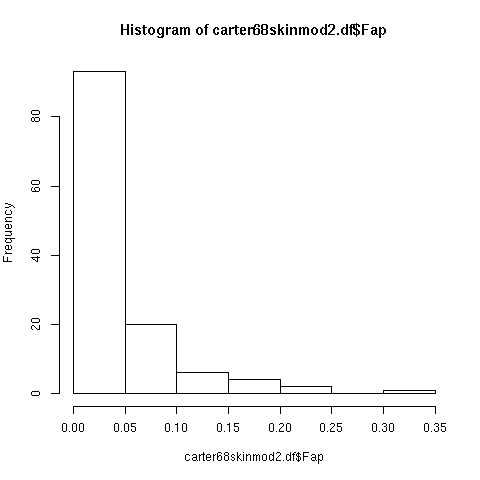
\includegraphics[width=0.9\textwidth]{faphist.png}
%  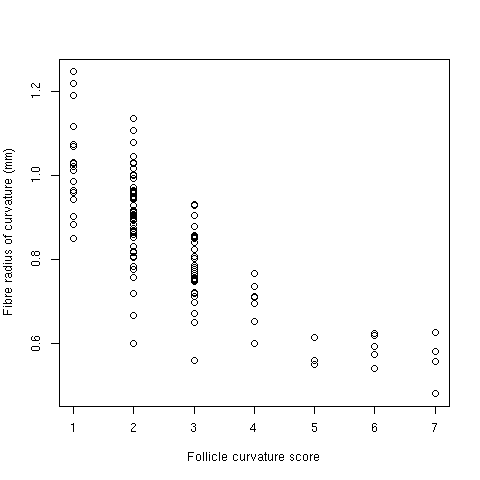
\includegraphics{ofdamm.png}
  \caption{Histogram of breed means for area of primary follicle tissue per $mm^{2}$ of skin at sebaceous gland level from data of Carter(1968)~\cite{cart:68}}
  \label{fig:faphist}
\end{figure}

%\end{document}


%\documentclass{article}
%\usepackage{graphicx,subfigure}
%\begin{document}

\begin{figure}[!h]
  \centering
   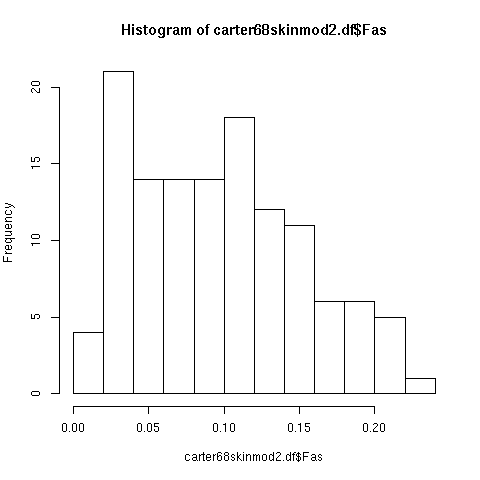
\includegraphics[width=0.9\textwidth]{fashist.png}
%  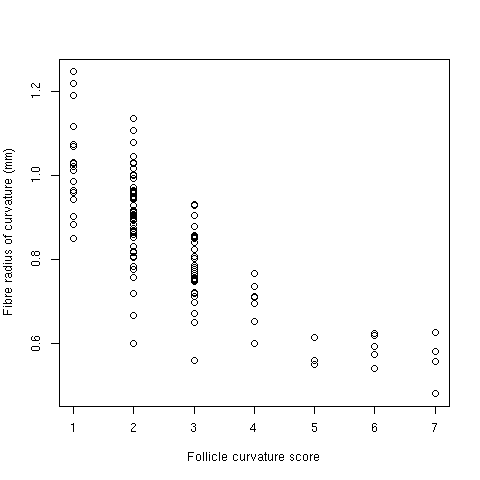
\includegraphics{ofdamm.png}
  \caption{Histogram of breed means for area of secondary follicle tissue per $mm^{2}$ of skin at sebaceous gland level from data of Carter(1968)~\cite{cart:68}}
  \label{fig:fashist}
\end{figure}

%\end{document}


We see a very considerable range in values for both $F_{ap}$ and $F_{as}$. A very small number of breeds have $F_{ap}$ larger than 0.10, whereas many breeds have $F_{as}$ larger than 0.10. 

We need to identify the breeds. This is done in Table~\ref{tab:fabreed}
% latex table generated in R 3.4.2 by xtable 1.8-2 package
% Tue Jan 30 20:57:23 2018
\begin{center}
%\begin{landscape}
\begin{longtable}{|p{1.0in}|p{2.0in}|p{1.0in}|p{1.0in}|}

\caption{Means of Fap and Fas for the Breeds of sheep sampled by Carter(1968)~\cite{cart:68}} \\
\hline
\label{tab:fabreed}
 & Breed & Fap & Fas \\ 
  \hline
1 &  Ak-karaman & 0.02 & 0.03 \\ 
\endfirsthead
\multicolumn{4}{c}%
{\tablename\ \thetable\ -- \textit{Continued from previous page}} \\
\hline
    & Breed  & Fap & Fas  \\ 
\hline
\endhead
\hline
\multicolumn{4}{r}{\textit{Continued on next page}} \\
\endfoot
\hline
\endlastfoot

  2 &  American Merino & 0.01 & 0.09 \\ 
  3 &  American Rambouillet & 0.01 & 0.13 \\ 
  4 &  Arabi & 0.04 & 0.04 \\ 
  5 &  Awassi & 0.04 & 0.04 \\ 
  6 &  Bellari White & 0.19 & 0.02 \\ 
  7 &  Bikaneri & 0.07 & 0.05 \\ 
  8 &  Blackhead Persian & 0.17 & 0.02 \\ 
  9 &  Black Kurumbai Adu & 0.10 & 0.03 \\ 
  10 &  Border Leicester & 0.04 & 0.10 \\ 
  11 &  Cheviot & 0.03 & 0.08 \\ 
  12 &  Chokla & 0.03 & 0.03 \\ 
  13 &  Columbia & 0.01 & 0.11 \\ 
  14 &  Corriedale & 0.02 & 0.15 \\ 
  15 &  Daglic & 0.05 & 0.06 \\ 
  16 &  Debouillet & 0.01 & 0.08 \\ 
  17 &  Dorset Horn & 0.02 & 0.13 \\ 
  18 &  Early Fine Merino & 0.01 & 0.12 \\ 
  19 &  Early Fine Merino (Rambouillet) & 0.01 & 0.13 \\ 
  20 &  English Leicester & 0.03 & 0.11 \\ 
  21 &  German Merinofleischaf & 0.01 & 0.09 \\ 
  22 &  German Merinolandschaf & 0.02 & 0.12 \\ 
  23 &  Icelandic & 0.05 & 0.06 \\ 
  24 &  Ile-de-France & 0.01 & 0.08 \\ 
  25 &  Improved Apulian & 0.01 & 0.08 \\ 
  26 &  Imroz & 0.08 & 0.08 \\ 
  27 &  Ivesi & 0.06 & 0.05 \\ 
  28 &  Jaisalmeri & 0.04 & 0.03 \\ 
  29 &  Kali & 0.04 & 0.03 \\ 
  30 &  Karakaya & 0.07 & 0.05 \\ 
  31 &  Karakul & 0.06 & 0.05 \\ 
  32 &  Kerradi & 0.04 & 0.03 \\ 
  33 &  Kivircik & 0.04 & 0.06 \\ 
  34 &  Limousin & 0.06 & 0.07 \\ 
  35 &  Lincoln & 0.05 & 0.12 \\ 
  36 &  Magra & 0.04 & 0.03 \\ 
  37 &  Malpura & 0.05 & 0.02 \\ 
  38 &  Mandya & 0.30 & 0.04 \\ 
  39 &  Marwari & 0.04 & 0.02 \\ 
  40 &  Merino Tor Mancina & 0.01 & 0.09 \\ 
  41 &  Navajo & 0.02 & 0.08 \\ 
  42 &  Nellore & 0.22 & 0.01 \\ 
  43 &  Nilgiri & 0.03 & 0.07 \\ 
  44 &  Non-Peppin Fine-Medium Merino & 0.01 & 0.15 \\ 
  45 &  Non-Peppin Medium Merino & 0.01 & 0.19 \\ 
  46 &  NSW Fine Merino & 0.01 & 0.17 \\ 
  47 &  Ossimi & 0.05 & 0.13 \\ 
  48 &  Ouda & 0.16 & 0.02 \\ 
  49 &  Peppin Medium Merino & 0.01 & 0.18 \\ 
  50 &  Polwarth & 0.01 & 0.14 \\ 
  51 &  Portuguese Merino & 0.01 & 0.08 \\ 
  52 &  Prealpes du Sud & 0.03 & 0.09 \\ 
  53 &  Rahmani & 0.04 & 0.12 \\ 
  54 &  Romney Marsh & 0.03 & 0.12 \\ 
  55 &  Ryeland & 0.01 & 0.07 \\ 
  56 &  Sakiz & 0.07 & 0.06 \\ 
  57 &  SA Strong Merino & 0.02 & 0.21 \\ 
  58 &  Scottish Blackface & 0.11 & 0.04 \\ 
  59 &  Soay & 0.05 & 0.03 \\ 
  60 &  Sonadi & 0.05 & 0.01 \\ 
  61 &  Sopravissano Rossi & 0.01 & 0.08 \\ 
  62 &  Southdown & 0.02 & 0.12 \\ 
  63 &  Suffolk & 0.02 & 0.06 \\ 
  64 &  Swaledale & 0.12 & 0.04 \\ 
  65 &  Swedish Landrace (Carpet) & 0.08 & 0.10 \\ 
  66 &  Swedish Landrace (Fine) & 0.04 & 0.12 \\ 
  67 &  Tanganyika Long-tailed & 0.13 & 0.01 \\ 
  68 &  Targhee & 0.01 & 0.12 \\ 
  69 &  Tas. Fine Merino & 0.01 & 0.15 \\ 
  70 &  Turkish Merino & 0.01 & 0.08 \\ 
  71 &  Vic. Fine Merino & 0.01 & 0.14 \\ 
  72 &  Welsh Mountain & 0.09 & 0.07 \\ 
  73 &  Wiltshire Horn & 0.07 & 0.08 \\ 
  74 &  Yankasa & 0.21 & 0.03 \\ 
   \hline
\end{longtable}
%\end{landscape}
\end{center}


and we collapse these breeds into Types in Table~\ref{tab:fatype}
% latex table generated in R 3.4.2 by xtable 1.8-2 package
% Tue Jan 30 21:03:37 2018
\begin{table}[ht]
\centering
\caption{Means of Fap and Fas for Types for sheep sampled by Carter(1968)~\cite{cart:68}}
\label{tab:fatype}
\begin{tabular}{rlrr}
  \hline
 & Type & Fap & Fas \\ 
  \hline
1 & African & 0.17 & 0.02 \\ 
  2 & Asian & 0.05 & 0.05 \\ 
  3 & Carpetwool & 0.11 & 0.05 \\ 
  4 & Cheviot & 0.03 & 0.08 \\ 
  5 & Corriedale & 0.02 & 0.15 \\ 
  6 & Downswool & 0.02 & 0.10 \\ 
  7 & Egyptian & 0.04 & 0.13 \\ 
  8 & European & 0.04 & 0.09 \\ 
  9 & Icelandic & 0.05 & 0.06 \\ 
  10 & Indian & 0.09 & 0.03 \\ 
  11 & Longwool & 0.04 & 0.11 \\ 
  12 & Merino & 0.01 & 0.14 \\ 
  13 & Polwarth & 0.01 & 0.14 \\ 
  14 & Soay & 0.05 & 0.03 \\ 
  15 & USA & 0.02 & 0.10 \\ 
  16 & Wiltshire & 0.07 & 0.08 \\ 
   \hline
\end{tabular}
\end{table}


Only the African and Indian hair sheep and the Carpetwools have $F_{ap}$ exceeding 0.10. 
The breeds with $F_{as}$ exceeding 0.10 are the Merino and Merino derived breedsplus the Egyptian  Ossimi and Rahmani. Neither of these Egyptian breeds seem to be wrinkled, but the Merino and its derivatives certainly can be wrinkled.

From these data Fas between 10 and 15 percent seems to be the cutoff point above which dermal expansion is too great and can lead to wrinkle. If the the follicles in a wrinkled sheep are 15-20 percent of the skin area, that means thet the amount of dermal expansion caused by the follicle formation can only be 15-20 percent. That seems a bit small to account for large folds. However, remember that $F_{as}$ is relative to a 1 $mm^{2}$ area after expansion has occurred. To check, we need a measure of dermal expansion. We attempt to develop that in the next section

Before we leave Fas and Fap, we should look at the relation between them. Figure~\ref{fig:fasfap} showns the relationship between means of all 126 flocks sampled by Carter(1968)~\cite{cart:68}. It would seem that sheep either have a lot of primary follicle tissue, or a lot of secondary follicle tissue, but not both. It would seem that the limit is about 30 percent of skin area consisting of follicle tissue, and this can be all primaries, nearly all secondaries, or a mixture.  This is a classic demonstration of the pre-papilla cell hypothesis (Moore etal (1998)~\cite{moor:98}). 
%\documentclass{article}
%\usepackage{graphicx,subfigure}
%\begin{document}

\begin{figure}[!h]
  \centering
   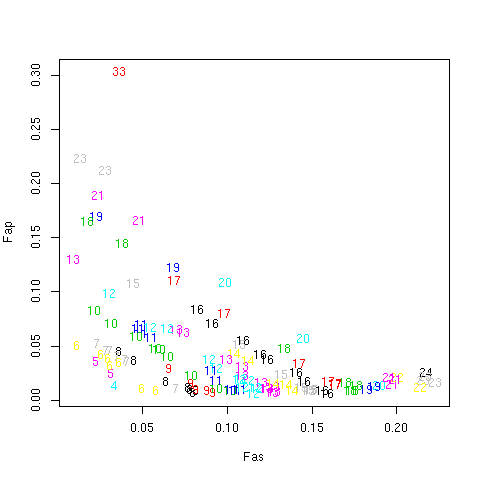
\includegraphics[width=0.9\textwidth]{fasfap.png}
%  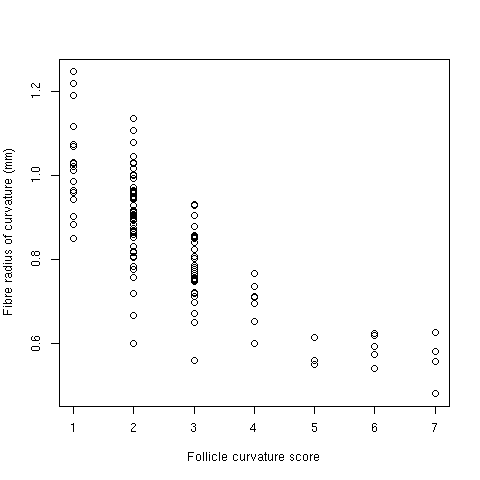
\includegraphics{ofdamm.png}
  \caption{Plot of flock means for area of secondary follicle tissue per $mm^{2}$ of skin against area of primary follicle tissue per $mm^{2}$ of skin for the 126 flocks sampled by Carter(1968)~\cite{cart:68}. The numbers representing each point are the total amount of follicle tissue per $mm^{2}$ of skin as a percentage.}
  \label{fig:fasfap}
\end{figure}

%\end{document}



\subsection{Using $N_{p}$ as a measure of dermal expansion}
It is often assumed that all sheep have the same density of primary follicles at the time when they initiate, and that subsequent differences in $N_{p}$ per unit area reflect differences in skin growth. Skin growth would include expansion of the dermis during secondary follicle initiation, as proposed here. 

It is therefore of interest to have a look at $N_{p}$ variation in the Carte(1968)~\cite{cart:68} data, and in particular to see if it is lower in breeds which exhibit wrinkle. 

Table~\ref{tab:nptype} shown the means of $N_{p}$ for the sheep type groupings of Carter(1968)~\cite{cart:68} and Table~\ref{tab:npbreed} shows the breed means. 
% latex table generated in R 3.4.2 by xtable 1.8-2 package
% Wed Jan 31 20:44:16 2018
\begin{table}[ht]
\centering
\caption{Means of $N_{p}$ for Types of sheep sampled by Carter(1969)~\cite{cart:68}}
\label{tab:nptype}
\begin{tabular}{rlr}
  \hline
 & Type & Npua \\ 
  \hline
1 & African & 3.40 \\ 
  2 & Asian & 2.37 \\ 
  3 & Carpetwool & 2.52 \\ 
  4 & Cheviot & 2.87 \\ 
  5 & Corriedale & 2.13 \\ 
  6 & Downswool & 3.14 \\ 
  7 & Egyptian & 3.00 \\ 
  8 & European & 2.13 \\ 
  9 & Icelandic & 1.50 \\ 
  10 & Indian & 3.64 \\ 
  11 & Longwool & 2.75 \\ 
  12 & Merino & 2.99 \\ 
  13 & Polwarth & 3.52 \\ 
  14 & Soay & 3.60 \\ 
  15 & USA & 1.87 \\ 
  16 & Wiltshire & 2.70 \\ 
   \hline
\end{tabular}
\end{table}


tex table generated in R 3.4.2 by xtable 1.8-2 package
% Wed Jan 31 20:48:35 2018
\begin{center}
%\begin{landscape}
\begin{longtable}{|p{1.0in}|p{2.0in}|p{1.0in}|}

\caption{Means of Np for the Breeds of sheep sampled by Carter(1968)~\c
ite{cart:68}} \\
\hline
\label{tab:npbreed}
 & Breed & Np  \\ 
  \hline
1 &  Ak-karaman & 1.80 \\
\endfirsthead
\multicolumn{3}{c}%
{\tablename\ \thetable\ -- \textit{Continued from previous page}} \\
\hline
    & Breed  & Np   \\ 
\hline
\endhead
\hline
\multicolumn{3}{r}{\textit{Continued on next page}} \\
\endfoot
\hline
\endlastfoot

  2 &  American Merino & 2.80 \\ 
  3 &  American Rambouillet & 2.40 \\ 
  4 &  Arabi & 2.10 \\ 
  5 &  Awassi & 1.90 \\ 
  6 &  Bellari White & 3.00 \\ 
  7 &  Bikaneri & 6.60 \\ 
  8 &  Blackhead Persian & 3.70 \\ 
  9 &  Black Kurumbai Adu & 3.60 \\ 
  10 &  Border Leicester & 3.00 \\ 
  11 &  Cheviot & 2.87 \\ 
  12 &  Chokla & 3.80 \\ 
  13 &  Columbia & 1.80 \\ 
  14 &  Corriedale & 2.13 \\ 
  15 &  Daglic & 2.90 \\ 
  16 &  Debouillet & 3.00 \\ 
  17 &  Dorset Horn & 2.90 \\ 
  18 &  Early Fine Merino & 4.00 \\ 
  19 &  Early Fine Merino (Rambouillet) & 3.45 \\ 
  20 &  English Leicester & 2.50 \\ 
  21 &  German Merinofleischaf & 2.10 \\ 
  22 &  German Merinolandschaf & 2.70 \\ 
  23 &  Icelandic & 1.50 \\ 
  24 &  Ile-de-France & 2.10 \\ 
  25 &  Improved Apulian & 2.30 \\ 
  26 &  Imroz & 3.20 \\ 
  27 &  Ivesi & 2.50 \\ 
  28 &  Jaisalmeri & 3.20 \\ 
  29 &  Kali & 3.10 \\ 
  30 &  Karakaya & 2.10 \\ 
  31 &  Karakul & 3.30 \\ 
  32 &  Kerradi & 1.50 \\ 
  33 &  Kivircik & 2.50 \\ 
  34 &  Limousin & 2.00 \\ 
  35 &  Lincoln & 2.53 \\ 
  36 &  Magra & 3.60 \\ 
  37 &  Malpura & 3.10 \\ 
  38 &  Mandya & 4.70 \\ 
  39 &  Marwari & 3.40 \\ 
  40 &  Merino Tor Mancina & 2.60 \\ 
  41 &  Navajo & 1.80 \\ 
  42 &  Nellore & 2.30 \\ 
  43 &  Nilgiri & 4.10 \\ 
  44 &  Non-Peppin Fine-Medium Merino & 2.25 \\ 
  45 &  Non-Peppin Medium Merino & 2.40 \\ 
  46 &  NSW Fine Merino & 3.40 \\ 
  47 &  Ossimi & 3.00 \\ 
  48 &  Ouda & 3.20 \\ 
  49 &  Peppin Medium Merino & 3.10 \\ 
  50 &  Polwarth & 3.52 \\ 
  51 &  Portuguese Merino & 3.10 \\ 
  52 &  Prealpes du Sud & 2.40 \\ 
  53 &  Rahmani & 3.00 \\ 
  54 &  Romney Marsh & 2.95 \\ 
  55 &  Ryeland & 2.10 \\ 
  56 &  Sakiz & 2.80 \\ 
  57 &  SA Strong Merino & 3.27 \\ 
  58 &  Scottish Blackface & 2.17 \\ 
  59 &  Soay & 3.60 \\ 
  60 &  Sonadi & 2.80 \\ 
  61 &  Sopravissano Rossi & 2.40 \\ 
  62 &  Southdown & 3.80 \\ 
  63 &  Suffolk & 3.50 \\ 
  64 &  Swaledale & 2.30 \\ 
  65 &  Swedish Landrace (Carpet) & 2.10 \\ 
  66 &  Swedish Landrace (Fine) & 1.80 \\ 
  67 &  Tanganyika Long-tailed & 3.30 \\ 
  68 &  Targhee & 2.00 \\ 
  69 &  Tas. Fine Merino & 2.96 \\ 
  70 &  Turkish Merino & 2.40 \\ 
  71 &  Vic. Fine Merino & 3.62 \\ 
  72 &  Welsh Mountain & 3.13 \\ 
  73 &  Wiltshire Horn & 2.70 \\ 
  74 &  Yankasa & 3.40 \\ 
   \hline
\end{longtable}
%\end{landscape}
\end{center}

There is no clear result. The Merino means are intermediate. Clearly growth differences are interfering with our attempt to use $N_{p}$ as an indicator of dermal expansion.

\subsection{Data on variation within a wrinkled Merino flock}
We have a set of data in which degree of wrinkle is actually recorded for each sheep as a scores for neck wrinkle and body wrinkle according to the photographic standards of Turner, etal (1953)~\cite{turn:53}. We also have skin histology measurements for these sheep, so we can calculate $F_{ap}$ and $F_{as}$. This flock is the CSIRO experimant known as AB32, for which genetic parameters are reported by Jackson(2017)~\cite{jack:17a}. There is also a summary of the genetic parameter estimates relevant to wrinkle score in Jackson and Watts(2017)~\cite{jack:17b}.

What we do here is extend the genetic parameter estimates to include $F_{ap}$ and $F_{as}$. 


\clearpage
\section{Discussion}





\clearpage
\begin{thebibliography}{99}

\bibitem{bogo:40}
 Bogolyubsky S.N. (1940) cited by Fraser A.S and Short B.F. (1960) The Biology of the Fleece. Animal Research Laboratories Technical Paper No 3. CSIRO Melbourne 1960.

\bibitem{brow:68}
Brown, G.H., and Turner, Helen Newton. (1968) Response to selection in Australian Merino sheep. II. Estimates of phenotypic and genetic parameters for some production traits in Merino ewes and an analysis of the possible effects of selection on them. Aust. J. Agric. Res. 19:303-22

\bibitem{cart:43}
Carter H.B. (1943) Studies in the biology of the skin and fleece of sheep. 1. The development and general histology of the follicle group in the skin of the Merino. 2. The use of tanned sheepskin in the study of follicle population density. 3. Notes on the arrangement, nomenclature, and variation of skin folds and wrinkles in the Merino. C.S.I.R. Bulletin No 164, Melbourne, 1943

\bibitem{cart:68}
Carter,H.B. (1968) Comparative Fleece Analysis Data for Domestic Sheep. The Principal Fleece Staple Values of Some Recognised Breeds. Agricultural Research Council, 1968

\bibitem{fras:60}
Fraser A.S and Short B.F. (1960) The Biology of the Fleece. Animal Research Laboratories Technical Paper No 3. CSIRO Melbourne 1960.

\bibitem{gord:08}
Gordon-Thompson, C., Botto, S.A., Cam, G.R., and Moore, G.P.H. (2008) Notch pathway gene expression and wool follicle cell fates. Aust. J. Exp. Agric. 48(5) 648-656

\bibitem{jack:75}
Jackson, N., Nay, T, and Turner, Helen Newton (1975) Response to selection in Australian Merino sheep. VII Phenotypic and genetic parameters for some wool follicle characteristics and their correlation with wool and body traits. Aust. J. Agric. Res. 26:937-57

\bibitem{jack:15}
Jackson, N. (2015) Genetic relationship betweeen skin and wool traits in Merino sheep. Incomplete manuscript.

\bibitem{jack:17}
Jackson, N. (2017) Genetics of primary and secondary fibre diameters and densities in Merino sheep. URL https://github.com/nevillejackson/atavistic-sheep/mev-rewrite/supplementary/genetic-parameters/psparam.pdf

\bibitem{jack:17a}
Jackson, N. (2017) Genetic relationship between skin and wool traits in Merino sheep. Part I Responses to selection and estimates of genetic parameters. URL https://github.com/nevillejackson/Fleece-genetics/tree/master/skinandfleeceparameters/ab3220/skinwool1.pdf

\bibitem{jack:90}
Jackson, N., Maddocks, I.G., Lax, J., Moore, G.P.M. and Watts, J.E. (1990) Merino Evolution, Skin Characteristics, and Fleece Quality. URL https://github.com/nevillejackson/atavistic-sheep/mev/evol.pdf 

\bibitem{jack:17b}
Jackson, N. and Watts, J.E. (2017) What is known about the genetics of wrinkle score in Merino sheep? URL https://github.com/nevillejackson/Fleece-genetics/wrinkle/wrinkle.pdf

\bibitem{knig:93}
Knight, K.R., Lepore, D.A., Horne, R.S., Ritz, M., Kumta, S. and O'Brian, B.M. (1993) Collagen content of uninjured skin and scar tissue in foetal and adult sheep. Int. J. Exp. Pathol. 74(6):583-591

\bibitem{madd:88}
Maddocks, I.G. and Jackson, N. (1988) Structural studies of sheep, cattle, and goat skin. CSIRO, Division of Aimal Production, Sydney.

\bibitem{ment:80}
Menton, D.N. and Hess, R.A. (1980) The ultrastructure of collagen in the dermis of tight-skin (Tsk) mutant mice. The Journal of Investigative Dermatology 74:139-147

\bibitem{mitc:84}
Mitchell, T.W. et al (1984) Wool Technology and Sheep Breeding, No IV, 200-206

\bibitem{moor:89}
Moore G.P.M., Jackson, N., and Lax, J. (1989) Evidence of a unique developmental mechanism specifying bot wool follicle density and fibre size in sheep selected for single skin and fleece characters. Genet. Res. Camb. 53:57-62

\bibitem{moor:98}
Moore, G.P.M., Jackson, N., Isaacs, K., and Brown, G (1998) J. Theoretical Biology 191:87-94

\bibitem{nay:66}
Nay, T. (1966) Wool follicle arrangement and vascular pattern in the Australian Merino. Aust. J. Agric. Res. 17:797-805

\bibitem{rprog:13}
R Core Team (2013). R: A language and environment for statistical
  computing. R Foundation for Statistical Computing, Vienna, Austria.
  ISBN 3-900051-07-0, URL http://www.R-project.org/.

\bibitem{ryde:68}
Ryder, M.L. and Stevenson, S.K.(1968) Wool Growth. Academic Press, London.


\bibitem{turn:56} 
Turner, Helen Newton (1956) Anim. Breed. Abstr. 24:87-118

\bibitem{turn:58}
Turner, Helen Newton(1958) Aust. J. Agric. Res. 9:521-52

\bibitem{turn:53}
Turner, Helen Newton, Hayman, R.H., Riches, J.H., Roberts, N.F., and Wilson, L.T. (1953) Physical definition of sheep and their fleece for breeding and husbandry studies: with particular reference to Merino sheep. CSIRO Div. Anim. Hlth. Prod. Div. Rept. No. 4 (Ser SW-2 mimeo)

\bibitem{turn:70}
Turner, Helen Newton, Brooker M.G. and Dolling, C.H.S (1970) Response to selection in Australian Merino sheep. III Single character selection for high and low values of wool weight and its components. Aust.J.Agric.Res. 21:955-84

\bibitem{watt:17}
Watts, J.E., Jackson, N., and Ferguson, K.A. (2017) Improvements in fleece weight weight and wool quality of Merino sheep selected visually for high fibre density and length. URL https://github.com/nevillejackson/SRS-Merino/Paper\_2\_Revised\_10\_November\_2017.docx 

\bibitem{watt:17b}
Watts, J.E. and Jackson, N. (2017) Is collagen quantity and properties involved in wrinkle formation and/or in follicle development? URL https://github.com/nevillejackson/SRS-Merino/tree/master/supplementary/copllagen/collagen.pdf

\bibitem{xavi:03}
Xavier, S.P., Gordon-Thomson, C. Wynn, P.C., McCullagh, P., Thomson, P.C., Tomkins, L., Mason, R.S., and Moore, G.P.M.(2003) Evidence that Notch and Delta expressions have a role in dermal condensate aggregation during wool follicle initiation. Experimental Dermatology, 22:656-681

\end{thebibliography}
\end{document}
